\section{The Developing Process}
\label{sec:mpt}

% A description and illustration of:

%     How do you interact as developers?

%     How is the team organized?

%     A complete description of stages and tools included in the CI/CD chains.
%         That is, including deployment and release of your systems.

%     Organization of your repositor(ies).
%         That is, either the structure of of mono-repository or organization of artifacts across repositories.
%         In essence, it has to be be clear what is stored where and why.

%     Applied branching strategy.

%     Applied development process and tools supporting it
%         For example, how did you use issues, Kanban boards, etc. to organize open tasks

%     How do you monitor your systems and what precisely do you monitor?

%     What do you log in your systems and how do you aggregate logs?

%     Brief results of the security assessment.

%     Applied strategy for scaling and load balancing.

% In essence it has to be clear how code or other artifacts come from idea into the running system and everything that happens on the way.

\subsection{Developer interaction}
Our main way of interacting with each other on a weekly basis has primarily been on the communication platform \textit{Discord}\footnote{\url{https://www.discord.gg}}. We have used this platform to not only communicate, but also share relevant articles, repositories and notes. This has worked pretty well, and we did not experience any issues with lack of communication within the team.\\

% Write about multiple channels on Discord maybe?
%Team communication. Where? What went well? What could have been better? Why?

This project included a large amount of tasks that we needed to keep track of and prioritise. We therefore decided to use \textit{GitHub Issues} along with the \textit{labels} that this service presented us with. This will be explained in greater detail in the next section. \\ 

%GitHub: Issues used to keep track of things (not in detail -> Team Organisation). GitHub Workflows for ci/cd (not in detail as this will be mentioned later)

Overall, we have experienced a good workflow, with only a few complications. We did however, experience difficulty with implementing logging, which led to the server crashing and caused panic within the team. This will be covered in section 3.7.

%team workflow and interaction with the project

\subsection{Team Organisation}

The team organisation has been playing a key part in our \textit{MiniTwit} project. Especially creating a structured approach to the organisation of tasks has proven to be an important functionality. This is due to the team having a lot of other projects and work running in parallel with this course, causing a quick loss of overview if not helped.

As mentioned in the previous section, one of the tools that has helped organising our effort has been \textit{GitHub Issues}. The Kanban board feature that \textit{GitHub Issues} makes use of has been the dashboard of productivity in our project, and has enabled us to quickly gain an overview of pending tasks and current progressing. As with most project organising tools, the ability to assign and prioritise tasks is powerful features that allows for distributing work with less effort and increase team-wide oversight.  


%How did the team stay organised? How did we keep track of new problems and communication while the simulator was running? (GitHub issues)
%Should we write anything about physical organisation of the teamwork?

\subsection{CI/CD Description}

All CI/CD related workflows are running through the use of \textit{GitHub Actions}. We made a total of six workflows:\footnote{\url{https://github.com/Faurby/BlackOps/tree/main/.github/workflows}}

\subsubsection{deployy.yml}
The deployment workflow is activated once there is a push to the main branch, which happens after a successful merge. First it logs into the \textit{DockerHub} account, which has our custom images, and then it pushes newest local images. After this it SSH into the root of our \textit{MiniTwit} droplet, which is running the application. Then it pulls git, pulls docker, and deploy our two updated stacks to the docker swarm.

We later realized, that there was no need to pull our entire code base to the droplet, as it only needed the two docker compose files to run our services. This could have been optimized, since unnecessary places for the code base to be, could lead to a higher security risk.

\subsubsection{dotnet.yml}
This is a simple template from \textit{GitHub Marketplace}, that tests your \textit{.NET} environment. It is activated on all pull requests to main.

\subsubsection{release.yml}
The release workflow was made to help ensure that we made at least one weekly release. The release workflow was made following a guide made by \textit{Cees-Jan Kiewiet} \footnote{\url{https://github.com/WyriHaximus/github-action-next-semvers}}. There were two ways of triggering this workflow: a minor release is made when pushing to main, and a major release is made on a cron job running every Sunday at 19. Unfortunately, we had some issues regarding the use of tags, and \textit{GitHub's} naming convention, leading to multiple issues regarding major releases. To fix this, we would need to find another way of incrementing the tags, while allowing for the possibility that a tag could already exist.

\subsubsection{snykimagescan.yml}
This workflow activates on pull requests to main. It logs into our \textit{DockerHub}, builds the custom images we have, and scans them for vulnerabilities. This is then displayed in the \textit{GitHub} pull requests.

\subsubsection{sonarcube.yml}
This workflow activates on pull requsts to main. It pushes our code to the \textit{SonarCloud} application, where it is scanned for vulnerabilities, code smells, warnings, etc. This is then displayed in the \textit{GitHub} pull request.

\subsubsection{yamllint.yml}
This is a simple workflow which is activated on pull requests to main. It scans our .yml files and finds wrong syntax. This is displayed in the \textit{GitHub} pull request.

We could improve a lot on our three workflows that scan our code base or docker images. At the current state, we have a very relaxed policy regarding errors and warnings. As long as it does not break the production, we don't prioritize fixing it. This could have been improved upon by having stricter policies. E.g., have a x score, x amount of warnings, before you could merge into main. This would optimize the quality of our code. 

% Go into detail about GitHub Actions

% What were our different yml files and what was the purpose of them? Could we have improved them, and if yes, how?

% Reflections and expansion: Considerations regarding new workflows. What could we have made to make our project even better

\subsection{Repository Organisation}
Our entire code base was stored in a single repository. This was mainly due to the initial template, but was also very convenient when deploying.


\subsection{Branching Strategy}

We chose to follow a trunk based management practice for this project. We tried to make small and frequent changes, and did our best to merge these into the main branch as quickly as possible. We did this to try and follow the principle of continuous delivery. This streamlined the DevOps process, ensuring no branches diverged too much, which allowed us to avoid large merge conflicts. Frequent merges to main also let us stress test our CI/CD pipeline and discover issues.

Branch protection rules were set up where pull requests to the main branch would require a review from someone else in the group. As such, the merging branches into main frequently also enforced frequent code reviews. Here automated tests implemented in the CI/CD pipeline would preemptively flag issues before a manual code review would be performed by another developer on the team. Code reviews were mostly performed immediately after the creation of a pull request. We attempted to avoid long lived branches, but exceptions to this did occur when working on larger features that would break functionality until they were fully implemented.

\subsection{Monitoring}

%How did we monitor our system? (Prometheus and Grafana)

For the monitoring of our system we decided to use \textit{Prometheus} and \textit{Grafana}. This setup allowed us to store and visualize custom metrics from our system.

\textit{Prometheus} is used for pulling data from the system and storing it as metrics. Among others, we kept track of a count on the current amount of users registered or the amount of errors per second/minute.

\textit{Grafana} is used for visualizing the data from \textit{Prometheus}. \textit{Grafana} has many different customizable options for creating different dashboards, which allows for a quick overview of the current status of the system.

%Decisions for dashboard functions, problems and reflections
Figure \ref{GrafanaDashboard} depicts our final dashboard, which helped us keep track of different metrics, including the two we found to be the most important: The average response time of our controller and the error rate. We chose these as we came to realize that the server could not keep up the amount of simulator requests. Therefore, we decided to monitor the response time against the error rate to ensure the health of the server. We had to upgrade the server on multiple occasions, as it was starting to get overwhelmed with the increased rate of requests. 

\begin{figure}[H]
    \centering
    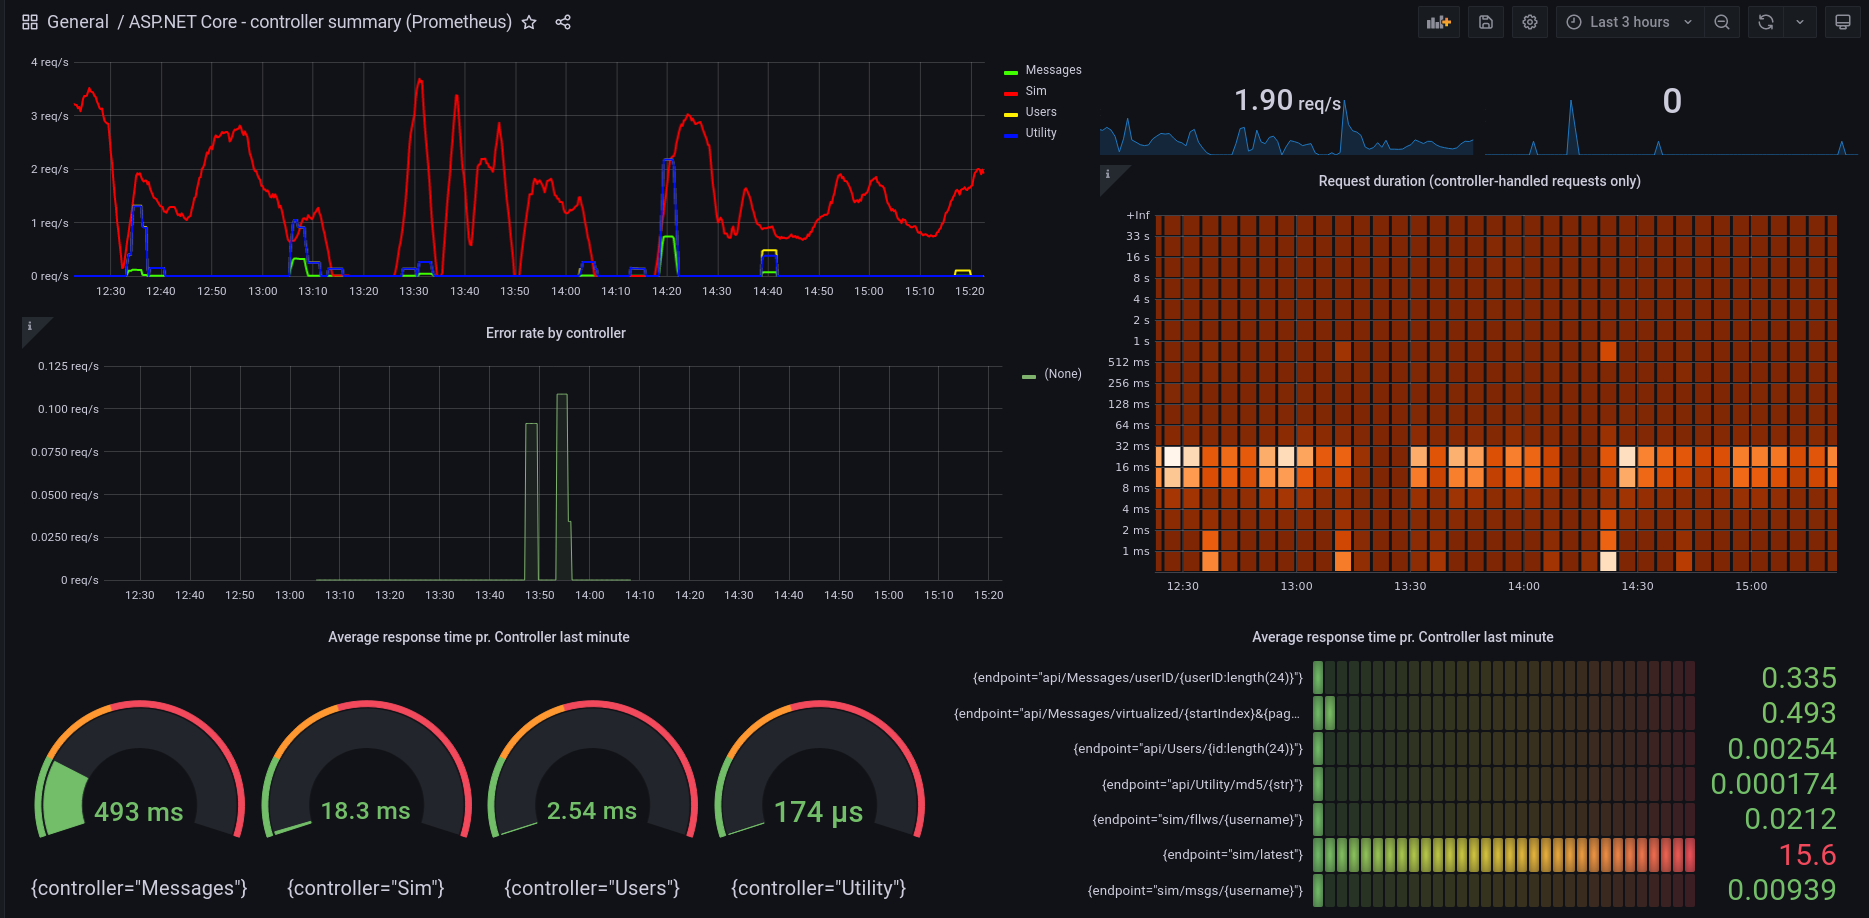
\includegraphics[width=16cm]{Diagrams/dashboard.png}
    \caption{Final version of our Grafana dashboard}
    \label{GrafanaDashboard}
\end{figure}

\subsection{Logging}
%Talk about serilogging(Don't think we ended up using serilogging), Nginx, Filebeat, Elastic Search and Kibana and logging in .NET.

%Also talk about how this led to our database getting deleted

%Further reflections / Improvements?
For implementing the logging of our system we added the ELK stack. This stack consist of the three open source products: \textit{Elasticsearch}, \textit{Logstash} and \textit{Kibana}. For added security to the ELK stack we decided on using \textit{Nginx} as a reverse proxy to redirect clients to the appropriate backend server. The ELK stack helps us by providing an easy to manage logging platform, which collects and processes all necessary logs.

\textit{Logstash} is used as a log aggregator, collecting logs from multiple parts of the code.

\textit{Elasticsearch} is used as a full-text search and analysis engine. 

\textit{Kibana} is a product used on top of Elasticsearch for visualizing data.

For getting the most optimized experience of the ELK stack, we could have added custom logs from our API endpoints. This would make it much easier to figure out when different errors, like the above mentioned, would occur and where to fix them.

\subsection{Security}

Using the security assessment we made\footnote{\url{https://github.com/Faurby/BlackOps/blob/main/Security\_Assessment.md}}, we found that our system was not completely secure. Exploring a couple of risk scenarios featuring some of the more common threats, we could establish a couple of flaws in our system. Some of the larger flaws included unwanted access to our database, as our connection string is openly available to anyone who knows the url of our \textit{GitHub} repository. Another issue is that passwords are openly available when using our API. At this given moment, we are trying to fix this by changing our \textbf{User} class to a \textbf{UserDTO}. This DTO will not have a password, thus eliminating the problem. The security evaluation made it very easy to find potential problems, and was something we were planning to do again, if the course ran for a longer period of time.
%Security assessment results (Probably needs to get shortened a bit)

\subsection{Scaling and load balancing}
To implement the possibility for scaling and load balancing, we use \textit{Docker Swarm}\footnote{\url{https://docs.docker.com/engine/swarm/}}. \textit{Docker Swarm} gives us the possibility to spawn multiple containers of the same image, and internally load balance incoming requests between these.

In its current state, our setup uses a single replica of each underlying system in our architecture, while our webserver has two replicas. This allows for an easier time updating the service, along with the absence of down time during an update. We have included a 10 second delay between updating the two webservers, to ensure that potentially harmful situations do not arise. 